\documentclass[border=10pt]{standalone}
\usepackage{tikz}
\usetikzlibrary{decorations.text}
\usepackage{xcolor}
\definecolor{myblue}{RGB}{0,0,170}
\definecolor{myred}{RGB}{170,0,0}
\definecolor{myorange}{RGB}{255,128,0}
\definecolor{mygreen}{RGB}{0,100,0}

\begin{document}
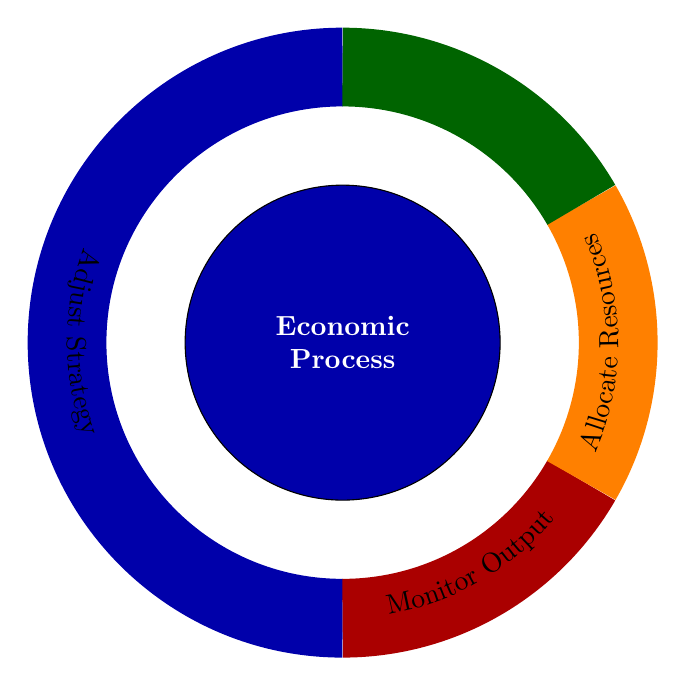
\begin{tikzpicture}[scale=1, transform shape]
    % Central circle
    \draw[fill=myblue] (0,0) circle (2cm);
    \node[white, font=\bfseries, text width=3cm, align=center] at (0,0) {Economic Process};
    
    % Blue segment: Adjust Strategy
    \draw[myblue, line width=1cm] (90:3.5cm) arc (90:270:3.5cm);
    \path[
        decorate,
        decoration={
            text along path,
            text={Adjust Strategy},
            text align=center,
            reverse path,
            text color=black
        }
    ] (270:3.5cm) arc (270:90:3.5cm);
    
    % Red segment: Monitor Output
    \draw[myred, line width=1cm] (270:3.5cm) arc (270:330:3.5cm);
    \path[
        decorate,
        decoration={
            text along path,
            text={Monitor Output},
            text align=center,
            text color=black
        }
    ] (270:3.5cm) arc (270:330:3.5cm);
    
    % Orange segment: Allocate Resources
    \draw[myorange, line width=1cm] (330:3.5cm) arc (330:390:3.5cm);
    \path[
        decorate,
        decoration={
            text along path,
            text={Allocate Resources},
            text align=center,
            text color=black
        }
    ] (330:3.5cm) arc (330:390:3.5cm);
    
    % Green segment (completing the circle)
    \draw[mygreen, line width=1cm] (30:3.5cm) arc (30:90:3.5cm);
\end{tikzpicture}
\end{document}